\documentclass[a4paper,12pt]{article}

\usepackage[utf8]{inputenc}
\usepackage[MeX]{polski}
\usepackage{fullpage}
\usepackage{graphicx}
\usepackage{hyperref}
\usepackage{tikz}
\usetikzlibrary{shapes.multipart,positioning}
\usepackage{fancyvrb}

\title{\LARGE{[SDPB] Wyznaczanie trasy} \\ \vspace{2mm} \large{Dokumentacja końcowa projektu}}
\author{Michał Aniserowicz, Jakub Turek}
\date{}

\begin{document}
	\maketitle

	\VerbatimFootnotes

	\section*{Temat projektu}

	Napisać aplikację wyznaczającą i~porównującą trasę przejazdu na terenie Warszawy środkami komunikacji miejskiej i~samochodem z~opcją ustawienia godziny wyjścia z~domu żeby zdążyć na czas. Aplikacja może być aplikacją mobilną lub przeznaczoną na komputer klasy PC.

	\section*{Założenia}

	Temat został uszczegółowiony poniższymi założeniami:

	\begin{itemize}
		\item Aplikacja zaprojektowana w~architekturze klient-serwer.
		\item Serwer posiada dwie odpowiedzialności:
		\begin{itemize}
			\item Przechowuje dane.
			\item Dostarcza logikę związaną z~przeliczaniem tras.
		\end{itemize}
		\item Klient jest aplikacją dostępową umożliwiającą wprowadzenie następujących danych:
		\begin{itemize}
			\item Lokalizacja początkowa i~docelowa (punkty na mapie).
			\item Docelowy czas przyjazdu.
			\item Przejazd komunikacją miejską lub samochodem.
		\end{itemize}
		\item Klient na wyjściu prezentuje najszybszą trasę dla podanych danych wejściowych oraz godzinę wyjścia/wyjazdu, która pozwala zdążyć na czas.
		\item Dane nie są dostarczane z~systemów zewnętrznych (np. \emph{Google Maps}, \emph{Jak dojadę}), ale składowane w~bazie danych opracowanej w~ramach projektu.
		\item Uproszczenie algorytmu wyznaczania trasy:
		\begin{itemize}
			\item Założenie, że czas przejazdu tego samego odcinka drogi komunikacją miejską i~samochodem jest identyczny.
			\item Brak uwzględnienia informacji o~godzinach przyjazdu środków komunikacji miejskiej na przystanki. Zakłada się, że czas wymagany na przesiadkę jest stały i~jest parametrem algorytmu.
			\item Wyznaczana jest zawsze pojedyncza najszybsza trasa dla wybranego środka komunikacji.
			\item Jako punkt początkowy i~końcowy wybierane są te lokalizacje spośród danych znajdujących się w~bazie, które są najbliższe lokalizacjom wskazanym przez użytkownika.
			\item W~przypadku wskazania komunikacji miejskiej jako środka transportu punktem początkowym i~końcowym podróży są zawsze przystanki najbliższe wskazanym lokalizacjom. Nie jest uwzględniana możliwość dojścia do przystanku.
		\end{itemize}
	\end{itemize}

	\section*{Model danych}

	W~aplikacji został wykorzystany sieciowy model danych:

	\begin{itemize}
		\item Miasto jest opisane przy pomocy węzłów oraz łuków:
			\begin{itemize}
				\item Współrzędne węzła (punkty) są opisane długością oraz szerokością geograficzną.
				\item Węzły opisują różne lokalizacje miejskie: przystanki autobusowe, skrzyżowania, etc.
				\item Łuki reprezentują połączenia drogowe pomiędzy węzłami. Są skierowane, więc można na nich opisać ruch jednokierunkowy.
				\item Informacja o~relacjach pomiędzy dwuwymiarowymi strukturami nie jest przechowywana.
			\end{itemize}
		\item Nie ma ograniczeń odnośnie planarności sieci: 
			\begin{itemize}
				\item Testowy zbiór danych jest siecią planarną.
				\item Aplikacja bez modyfikacji zadziała dla sieci nieplanarnych (tunele, przejazdy wielokondygnacyjne).
			\end{itemize}
	\end{itemize}

	\subsection*{Reprezentacja logiczna modelu danych}

	Relacyjny model baz danych nie jest dobrze przystosowany do opisu modelu sieciowego. Informacje o~stukturze grafowej można przechowywać na dwa sposoby:

	\begin{itemize}
		\item W~postaci znormalizowanych tabel - osobne tabele dla wierzchołków i~krawędzi.
		\item W~postaci zdenormalizowanych tabel - rekord tabeli zawiera pełną informację o~węźle i~wszystkich połączonych z~nim węzłach (wejściowych i~wyjściowych). Węzły wyjściowe i~wejściowe przechowywane są w~postaci dwóch osobnych list.
	\end{itemize}

	W~przypadku drugiego podejścia problemem jest przechowywanie informacji o~koszcie danej krawędzi. Wymaga ona opakowania informacji w~słownikową strukturę danych, co z~kolei uniemożliwia wykonywanie zapytań języka SQL. Alternatywą może być przechowywanie tylko informacji o~ścieżkach. Przy tym podejściu każdy rekord zawiera pełne informacje o~węźle początkowym i~końcowym. Jest to jednak duży narzut pamięciowy, gdyż informacja o~każdym węźle jest przechowywana $n$ razy, gdzie $n$ to stopień danego węzła.

	Algorytm wyszukiwania połączeń w~sieci wymaga dokonania wielu złączeń. Przykładowo dla postaci znormalizowanej, po wejściu do każdego węzła musimy najpierw pobrać informację o~łukach, które ten węzeł tworzy, a~następnie pobrać informacje o~połączonych z~nim węzłach. Jeżeli na etapie oszacowania kosztu potrzebna jest informacja o~węzłach poprzedzających, wtedy wykonywane będą kolejne złączenia. Jest to istotny narzut obliczeniowy. Zakładając, że w~ramach modelu danych będzie ujęte wiele typów relacji problem potęguje się.

	Opisany w~powyższym akapicie narzut nie wyklucza wykorzystania relacyjnej bazy danych do rozwiązania zadanego problemu. Autorzy projektu postanowili jednak skorzystać z~innego podejścia i~wykorzystać bazy danych o~reprezentacji logicznej lepiej nadającej się do modelowania dziedziny problemu.

	Interesującą alternatywę zapewnia ruch \textbf{Not Only SQL}, a~konkretnie jego podzbiór - grafowe bazy danych. Ich logiczny model danych jest spójny z~sieciowym modelem struktury miasta, dlatego bardzo dobrze nadają się do rozwiązania postawionego problemu. Jednym z~najbardziej dojrzałych projektów grafowych baz danych jest \textbf{Neo4j} (\url{http://www.neo4j.org}). Zaletą tej bazy w~kontekście tematyki przestrzennych baz danych jest posiadanie warstwy abstrakcji do obliczeń przestrzennych - \textbf{Neo4j Spatial}. Ze względu na wymienione zalety i~odpowiedniość struktury do dziedziny problemu, do implementacji projektu autorzy skorzystali właśnie z~tej bazy danych.

	\section*{Schemat modelu danych miasta}

	Wykorzystany model danych został schematycznie przedstawiony na rysunku~\ref{fig:data_model}.

	\begin{figure}[ht!]
		\centering
		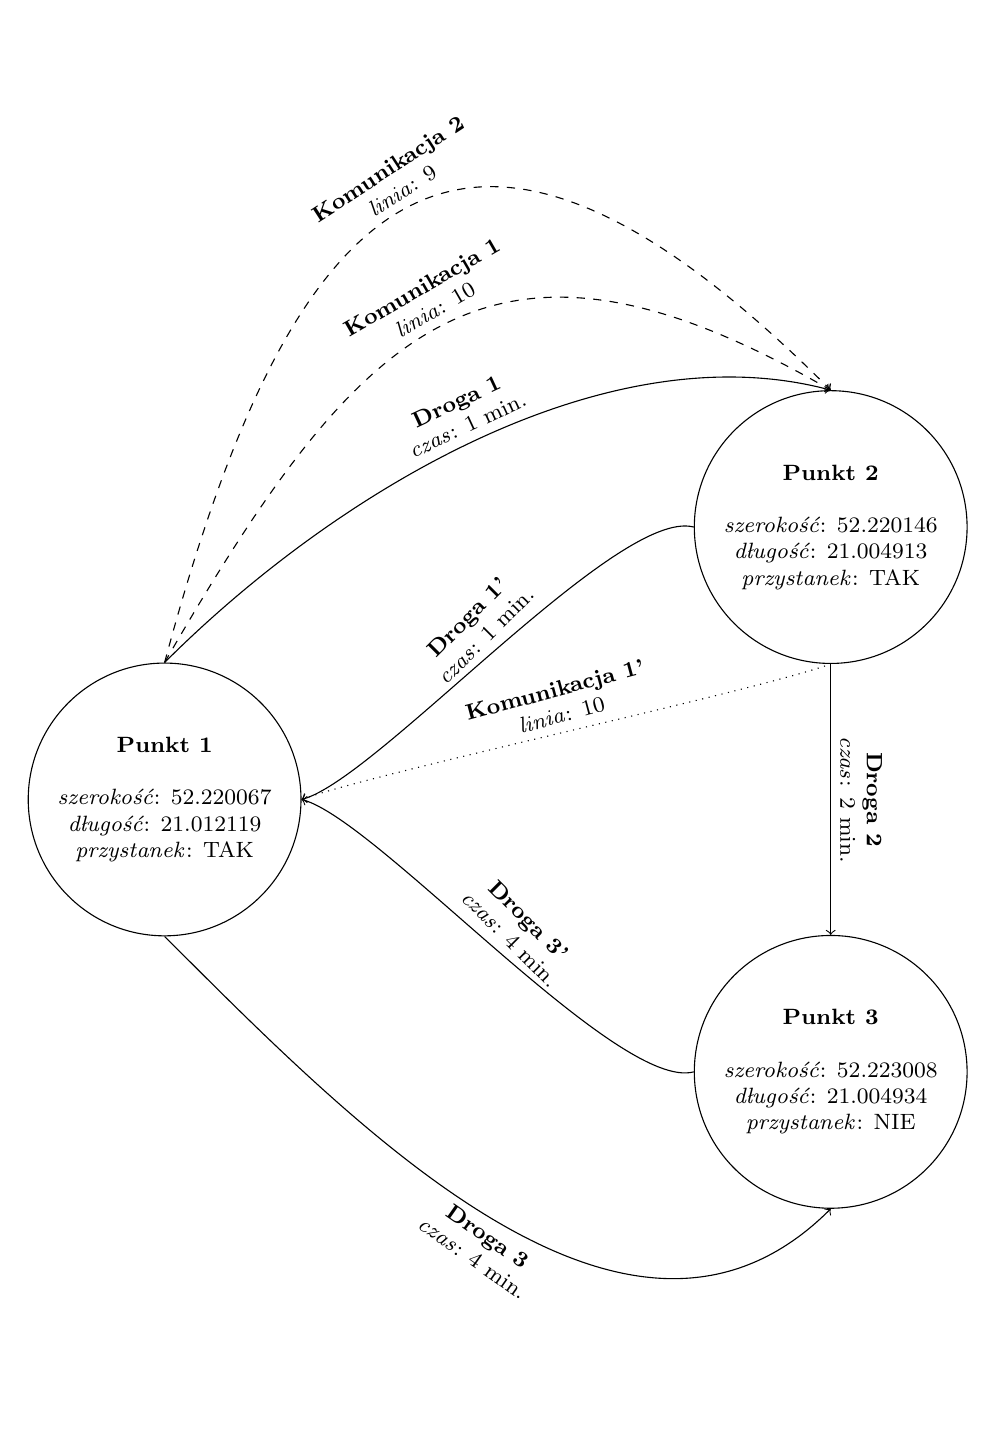
\begin{tikzpicture}[every text node part/.style={align=center,font=\footnotesize}]
			\node [draw, circle] (1) {{\bfseries Punkt 1} \\ \\ \emph{szerokość}: 52.220067 \\ \emph{długość}: 21.012119 \\ \emph{przystanek}: TAK};
			\node [draw, circle, above right=of 1, xshift=5cm] (2) {{\bfseries Punkt 2} \\ \\ \emph{szerokość}: 52.220146 \\ \emph{długość}: 21.004913 \\ \emph{przystanek}: TAK};
			\node [draw, circle, below right=of 1, xshift=5cm] (3) {{\bfseries Punkt 3} \\ \\ \emph{szerokość}: 52.223008 \\ \emph{długość}: 21.004934 \\ \emph{przystanek}: NIE};
			\draw [->, out=45, in=165, distance=3cm] (1.north) to node[above, rotate=25]{{\bfseries Droga 1} \\ \emph{czas}: 1 min.} (2.north);
			\draw [->, out=60, in=150, dashed, distance=5cm] (1.north) to node[above, rotate=30]{{\bfseries Komunikacja 1} \\ \emph{linia}: 10} (2.north);
			\draw [->, out=75, in=135, dashed, distance=6.5cm] (1.north) to node[above, rotate=33]{{\bfseries Komunikacja 2} \\ \emph{linia}: 9} (2.north);
			\draw [<-, out=15, in=165, distance=1cm] (1.east) to node[above, rotate=45]{{\bfseries Droga 1'} \\ \emph{czas}: 1 min.} (2.west);
			\draw [<-, out=20, in=200, distance=1cm, dotted] (1.east) to node[above, rotate=15]{{\bfseries Komunikacja 1'} \\ \emph{linia}: 10} (2.south);
			\draw [->, out=-45, in=-135] (1.south) to node[below, rotate=-35]{{\bfseries Droga 3} \\ \emph{czas}: 4 min.} (3.south);
			\draw [<-, out=-15, in=-165, distance=1cm] (1.east) to node[above, rotate=-45]{{\bfseries Droga 3'} \\ \emph{czas}: 4 min.} (3.west);
			\draw [->] (2.south) to node[above, rotate=-90]{{\bfseries Droga 2} \\ \emph{czas}: 2 min.} (3.north);
		\end{tikzpicture}

		\caption{Schematyczne przedstawienie modelu danych miasta.}
		\label{fig:data_model}
	\end{figure}

	Na schemacie pokazane są trzy punkty:

	\begin{enumerate}
		\item O~współrzędnych $(52.220067,21.012119)$. Przystanek komunikacji miejskiej.
		\item O~wpółrzędnych $(52.220146,21.004913)$. Przystanek komunikacji miejskiej.
		\item O~współrzędnych $(52.223008,21.004934)$.
	\end{enumerate}

	Na schemacie pokazane są dwa typy relacji. Relacja narysowana pełną linią o~nazwie \textbf{Droga} oznacza istnienie drogi pomiędzy punktami. Relacja narysowana linią przerywaną o~nazwie \textbf{Komunikacja} oznacza natomiast istnienie ścieżki przejazdu komunikacji miejskiej jednej linii pomiędzy tymi punktami. Z~relacji przedstawionych na schemacie można więc odczytać:

	\begin{itemize}
		\item Z~punktu~$1$ do punktu~$2$ prowadzi droga~$1$, której przebycie zajmuje jedną minutę. Istnieje droga powrotna~$1'$, która prowadzi z~punktu~$2$ do punktu~$1$. 
		\item Z~punktu~$1$ do punktu~$2$ można dojechać dwoma liniami komunikacji miejskiej: $9$~i~$10$. Z~punktu $2$ do punktu $1$ wraca tylko linia numer $10$.
		\item Punkty $2$ i~$3$ połączone są drogą jednokierunkową, której przebycie zajmuje 2~minuty.
		\item Punkty $1$ i~$3$ są połączone drogą dwukierunkową, której przejechanie zajmuje 4~minuty.
	\end{itemize}

	\subsection*{Indeksy}

	W~modelu danych założone są dwa indeksy:

	\begin{itemize}
		\item Indeks bitmapowy na polu \emph{przystanek}.
		\item Indeks przestrzenny na polach \emph{szerokość} i~\emph{długość} geograficzna\footnote{W~bazie danych Neo4j punkt jest reprezentowany jako łańcuch znaków WKT (Well-Known Text). Przykład: \verb+POINT( 52,223008 21,004934 )+.}.
	\end{itemize}

	\section*{Metoda wyznaczania trasy}

	Algorytm wyznaczania najszybszej trasy jest dwukrokowy:

	\begin{enumerate}
		\item W~bazie danych odnajdywane są dwa punkty: najbliższe początkowi i~końcowi trasy spośród wszystkich punktów zdefiniowanych w~bazie danych. W~przypadku wyznaczania trasy komunikacji miejskiej wyznaczane są takie najbliższe punkty, że są one przystankami komunikacji.
		\item Za pomocą algorytmu Dijkstry wyznaczana jest najszybsza droga pomiędzy znalezionymi punktami:
			\begin{itemize}
				\item Dla trasy samochodowej/pieszej pod uwagę brane są tylko i~wyłącznie łuki, które reprezentują relację \textbf{Droga}. Ewaluacja kosztu polega na dodawaniu czasu podróży dla każdego segmentu drogi.
				\item Dla podróży komunikacją miejską pod uwagę brane są tylko i~wyłącznie łuki, które reprezentują relację \textbf{Komunikacja}. Dla każdego segmentu wykonywana jest ewaluacja kosztu:
					\begin{itemize}
						\item Koszt jest zwiększany o~czas podróży dla danego segmentu.
						\item Wykonywane jest sprawdzenie czy do węzła wejściowego analizowanego łuku prowadzi łuk, który obsługuje ta sama linia komunikacyjna. Jeżeli tak to przesiadka jest zbędna i~ewaluacja kosztu kończy się. W~przeciwnym razie koszt całkowity ścieżki jest powiększany o~zadany czas oczekiwania na przesiadkę.
					\end{itemize}
			\end{itemize}
	\end{enumerate}

	\section*{Architektura aplikacji}

	Aplikacja została zaprojektowana w~architekturze klient-serwer. Szczegółowy schemat architektury przedstawia rysunek~\ref{fig:architecture}. 

	\begin{figure}[ht!]
		\centering
		\scalebox{0.7}[1.0]{
			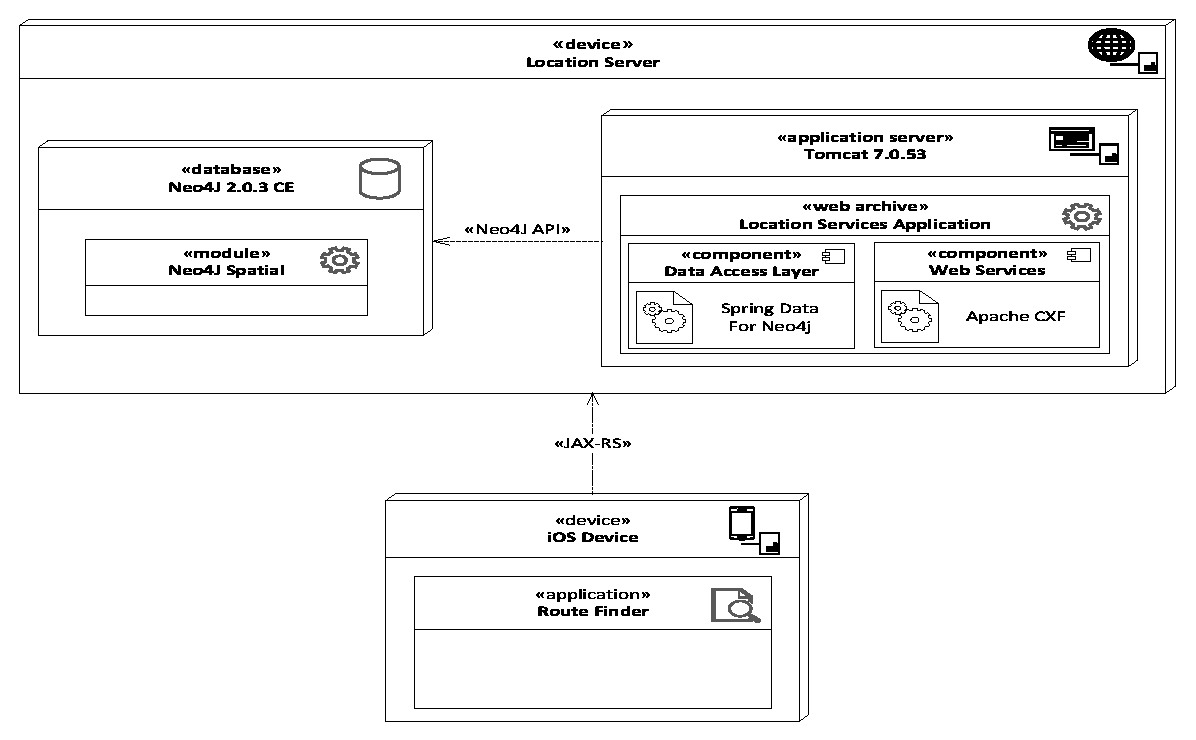
\includegraphics{graphics/architecture.eps}
		}

		\caption{Schemat architektury aplikacji.}
		\label{fig:architecture}
	\end{figure}

	\subsection*{Serwer}

	Serwer posiada następujące odpowiedzialności:

	\begin{itemize}
		\item Przechowuje informacje o~sieci miasta.
		\item Zwraca informacje o~najbliższych punktach z~bazy danych dla danej szerokości i~długości geograficznej\footnote{Przeszukiwanie domyślnie ograniczone jest do promienia 5~kilometrów. Ograniczenie to można zmienić w~pliku \verb+config.properties+.}.
		\item Zwraca informacje o~najbliższych przystankach komunikacji z~bazy danych dla danej szerokości i~długości geograficznej\footnotemark[2].
		\item Zwraca informacje o~najszybszej ścieżce dotarcia z~punktu o~identyfikatorze~A do punktu o~identyfikatorze~B. W~zależności od wywołania metody zwracana jest ścieżka dla samochodu lub komunikacji miejskiej.
	\end{itemize}

	\subsection*{Klient}

	Klient posiada następujące odpowiedzialności:

	\begin{itemize}
		\item Pozwala zdefiniować punkt początkowy i~końcowy podróży poprzez zaznaczenie na mapie.
		\item Umożliwia wprowadzenie godziny przyjazdu.
		\item Rysuje najszybszą ścieżkę na mapie na podstawie informacji pobranych z~serwera.
		\item Oblicza czas wyjścia z~domu na podstawie obecnego czasu i~długości podróży odebranej z~serwera.
		\item Pozwala na określenie czasu przesiadki.
	\end{itemize}

	\subsection*{Zasilanie danymi}

	Aby ułatwić inicjalne zasilanie bazy danych serwera utworzony został moduł o~nazwie \textbf{data-populator}:

	\begin{itemize}
		\item Moduł ten wypełnia bazę danych wartościami pobranymi ze zdefiniowanego repozytorium.
		\item Domyślnym repozytorium są trzy pliki płaskie, które odpowiednio zawierają informacje o~węzłach mapy, łukach dróg oraz łukach komunikacji miejskiej.
	\end{itemize}

	Rysunek~\ref{vrb:entries_repository} przedstawia przykład pliku definiującego punkty wejściowe dla węzłów mapy. Linie rozpoczynające się od znaku \textbf{\#} są traktowane jako komentarz. Kolejne kolumny oznaczają: identyfikator punktu w~obrębie repozytorium, szerokość geograficzną, długość geograficzną oraz flagę oznaczającą czy dany punkt jest przystankiem komunikacji miejskiej. Ostatnia kolumna, w~której znajduje się opis punktu, nie jest wprowadzana do bazy danych.

	\begin{figure}[ht!]
		\centering
		\begin{BVerbatim}
# id    latitude  longitude pt_stop description 
EN_0001 52.220067 21.012119 true    Plac Politechniki
EN_0002 52.220146 21.004913 true    Nowowiejska/Al. Niepodległości
EN_0003 52.223008 21.004934 true    Koszykowa/Chałubińskiego
EN_0004 52.227885 21.001865 true    Al. Jerozolimskie/Jana Pawła
EN_0005 52.230014 21.011886 true    Marszałkowska/Al. Jerozolimskie
EN_0006 52.219893 21.018152 true    Plac Zbawiciela
EN_0007 52.223232 21.015984 true    Plac Konstytucji
EN_0008 52.226229 21.014161 true    Marszałkowskiej/Hoża
EN_0009 52.228353 21.010203 false   Nowogrodzka/Poznańska
		\end{BVerbatim}
		\caption{Plik repozytorium zawierający dane wejściowe dla węzłów mapy.}
		\label{vrb:entries_repository}
	\end{figure}

	Rysunek~\ref{vrb:routes_repository} przedstawia przykład pliku definiującego łuki reprezentujące drogi. Kolumny oznaczają kolejno: identyfikator drogi w~obrębie repozytorium, identyfikator węzła początkowego drogi, identyfikator węzła końcowego drogi oraz czas podróży podany w~sekundach.

	\begin{figure}[ht!]
		\centering
		\begin{BVerbatim}
# id    from    to      travel_time_in_sec
RO_0001 EN_0001 EN_0002 180
RO_0002 EN_0002 EN_0003 120
RO_0003 EN_0003 EN_0004 240
RO_0004 EN_0004 EN_0005 300
RO_0005 EN_0001 EN_0006 120
RO_0006 EN_0006 EN_0007 120
RO_0007 EN_0007 EN_0008 120
RO_0008 EN_0008 EN_0005 240
		\end{BVerbatim}
		\caption{Plik repozytorium zawierający dane wejściowe dla łuków reprezentujących drogi.}
		\label{vrb:routes_repository}
	\end{figure}

	Rysunek~\ref{vrb:ptroutes_repository} przedstawia przykład pliku definiującego łuki reprezentujące transport publiczny. Kolumny oznaczają kolejno: identyfikator wpisu w~obrębie repozytorium, numer linii komunikacji oraz identyfikator drogi, po której porusza się komunikacja.

	\begin{figure}[ht!]
		\centering
		\begin{BVerbatim}
# id      line route
PTRO_0001 10   RO_0001
PTRO_0002 10   RO_0002
PTRO_0003 10   RO_0003
PTRO_0004 9    RO_0004
PTRO_0005 15   RO_0005
PTRO_0006 15   RO_0006
PTRO_0007 15   RO_0007
PTRO_0008 15   RO_0008
		\end{BVerbatim}
		\caption{Plik repozytorium zawierający dane wejściowe dla łuków reprezentujących komunikację publiczną.}
		\label{vrb:ptroutes_repository}
	\end{figure}	

	\subsection*{Komunikacja}

	Komunikacja odbywa się przy pomocy serwisów w~specyfikacji JAX-RS\footnote{Java API for RESTful Web Services.}. Zostały zdefiniowane dwa serwisy.

	\paragraph{Najbliższy punkt na mapie}

	Metoda jest dostępna przez odwołanie do relatywnej ścieżki \Verb+/nearest/{lat}/{lon}/publicTransportStop/{stop}+. Parametr \Verb+lat+ należy zastąpić szerokością geograficzną w~formacie zmiennoprzecinkowym z~kropką. Parametr \Verb+lon+ należy zastąpić długością geograficzną w~tym samym formacie. Parametr \Verb+stop+ należy natomiast wypełnić wartością \Verb+true+ lub \Verb+false+ jeżeli odpowiednio ma zostać zwrócony przystanek komunikacji miejskiej lub dowolny punkt. Serwis zwraca odpowiedź w~formacie przedstawionym na rysunku~\ref{vrb:entry_service_response}.

	\begin{figure}[ht!]
		\centering
		\begin{BVerbatim}
{
  "id": 15,
  "latitude": 52.219893,
  "longitude": 21.018152
}
		\end{BVerbatim}
		\caption{Przykładowa odpowiedź serwisu odnajdującego najbliższy punkt w~bazie danych.}
		\label{vrb:entry_service_response}
	\end{figure}	

	\paragraph{Najszybsza droga}

	Metoda może być wywołana poprzez odwołanie do relatywnej ścieżki \Verb+/shortestPath/{sId}/{fId}/publicTransport/{pT}/changeDuration/{cD}+. Parametr \Verb+sId+ należy zastąpić poprzez identyfikator węzła początkowego. Parametr \Verb+fId+ należy zastąpić poprzez identyfikator węzła końcowego. Oba identyfikatory mogą pochodzić z~wywołania serwisu dla najbliższego punktu na mapie. Parametr \Verb+pT+ należy zastąpić wartością \Verb+true+ lub \Verb+false+ w~zależności od tego czy wyszukana ma być droga dla komunikacji miejskiej lub samochodu. Ostatni parametr \Verb+cD+ należy zastąpić liczbą całkowitą, która oznacza ilość sekund doliczanych na oczekiwanie przy przesiadce. Odwołanie do \Verb+/changeDuration/{cD}+ jest opcjonalne dla najszybszej ścieżki samochodowej i~można je pominąć. Serwis zwraca odpowiedź w~formacie przedstawionym na rysunku~\ref{vrb:entry_service_response}.

	\begin{figure}[ht!]
		\centering
		\begin{BVerbatim}
[
  {
    "id": 10,
    "routeFrom": {
      "id": 15,
      "latitude": 52.219893,
      "longitude": 21.018152
    },
    "routeTo": {
      "id": 329,
      "latitude": 52.220067,
      "longitude": 21.012119
    },
    "duration": 300,
    "line": 9
  },
  {
    "id": 73,
    "routeFrom": {
      "id": 329,
      "latitude": 52.220067,
      "longitude": 21.012119
    },
    "routeTo": {
      "id": 412,
      "latitude": 52.228353,
      "longitude": 21.010203
    },
    "duration": 240,
    "line": 15
  }
]
		\end{BVerbatim}
		\caption{Przykładowa odpowiedź serwisu odnajdującego najszybszą ścieżkę pomiędzy punktami.}
		\label{vrb:entry_service_response}
	\end{figure}	

	\section*{Budowanie i~uruchamianie aplikacji}

	Moduł serwerowy oraz kliencki aplikacji budowane są osobno. Część serwerowa jest budowana przy użyciu aplikacji Maven (\url{http://maven.apache.org}). Uruchomienie polecenia \textbf{mvn clean install} w~ścieżce projektu spowoduje ściągnięcie wszystkich zależności, uruchomienie testów jednostkowych oraz integracyjnych, a~także wygenerowanie pliku web-archive (\textbf{.war}), który następnie trzeba \emph{zdeployować} na serwer aplikacji Java.

	Budowanie aplikacji klienckiej jest realizowane przy pomocy menadżera zależności CocoaPods (\url{http://cocoapods.org}). Uruchomienie polecenia \textbf{pod install} w~podfolderze z~klientem spowoduje ściągnięcie wszystkich zależności oraz wygenerowanie pliku projektu programu Xcode, za pomocą którego można skompilować i~wyeksportować aplikację.

	\section*{Implementacja}

	\subsection*{Moduły}

	Kod źródłowy projektu został podzielony na cztery moduły:

	\begin{description}
		\item[data-populator] służy do wypełniania bazy danych inicjalnymi wartościami. Odczytuje wartości z~plików płaskich.
		\item[data-access] interfejs abstrahujący dostęp do danych.
		\item[web-services] moduł udostępniający dostęp do bazy danych z~użyciem serwisów REST.
		\item[ios-client] aplikacja kliencka.
	\end{description}

	\subsection*{Środowisko uruchomieniowe}

	Projekt był uruchamiany i~testowany w~następującym środowisku:

	\begin{itemize}
		\item System operacyjny: OS X Mavericks 10.9.3 (dla aplikacji serwerowej), iOS 7.1.1 (dla aplikacji klienckiej).
		\item Wirtualna maszyna Java: JRE 1.8.0.
		\item Serwer aplikacyjny: Apache Tomcat 7.0.53.
		\item Baza danych: Neo4j 2.0.2 CE.
	\end{itemize}

	Kod źródłowy projektu (części serwerowej) jest zgodny z~najnowszą specyfikacją języka Java w~wersji 8. Wykorzystywane elementy języka to między innymi wskaźniki na funkcje, wyrażenia lambda oraz nowy interfejs programistyczny dla dat. Z~tego względu aplikacja nie uruchomi się w~starszej wersji maszyny wirtualnej.

	\subsection*{Środowisko developerskie}

	Projekt był implementowany przy użyciu:

	\begin{itemize}
		\item IntelliJ IDEA Ultimate 13.1.2. Zaawansowane IDE do programowania w~języku Java.
		\item Xcode 5.1.1. Domyślne IDE dla użytkowników systemu OS X umożliwiające tworzenie aplikacji na systemy OS X / iOS.
	\end{itemize}

	\subsection*{Testy jednostkowe}

	Projekt posiada zestaw testów jednostkowych, które pokrywają wszystkie moduły zaimplementowane na potrzeby tematu:

	\begin{itemize}
		\item Testy jednostkowe operacji bazodanowych z~wykorzystaniem biblioteki testującej dla Spring Data.
		\item Testy jednostkowe modułu wczytującego i~wypełniającego bazę danych inicjalnymi wartościami.
		\item Testy integracyjne serwisów, które automatycznie uruchamiają serwer aplikacyjny, uruchamiają na nim serwisy i~przeprowadzają testy klienckie.
		\item Testy jednostkowe komunikacji z~serwisami po stronie aplikacji klienckiej.
	\end{itemize}

	\subsection*{Wykorzystane oprogramowanie stron trzecich}

	Projekt wykorzystuje liczne elementy oprogramowania stron trzecich:

	\begin{itemize}
		\item JUnit 4.1.1. Biblioteka umożliwiająca testowanie jednostkowe aplikacji w~języku Java.
		\item Apache Maven 3.2.1. Narzędzie służy do budowania części serwerowej aplikacji. Pozwala na zarządzanie zależnościami i~przenośne budowanie projektu bez potrzeby dostarczania skompilowanych zależności wraz ze źródłami projektu.
		\item Spring Framework 4.0.3.RELEASE. Zestaw bibliotek programistycznych o~szerokim zakresie funkcjonalności do tworzenia aplikacji enterprise opartych o~język Java. W~projekcie wykorzystywany jest głównie jako kontener DI\footnote{Dependency Injection - wzorzec architektoniczny polegający na usuwaniu bezpośrednich zależności między komponentami.}.
		\item Neo4j API 2.0.2. Interfejs programistyczny dla języka Java umożliwiający korzystanie z~bazy danych Neo4j.
		\item Neo4j Spatial 0.12. Moduł dla bazy danych Neo4j do realizacji operacji i~indeksów przestrzennych. 
		\item Spring Data Neo4j 3.0.1.RELEASE. Wtyczka dla Spring Framework, która realizuje mapowanie obiektowe komponentów grafowej bazy danych Neo4j.
		\item Apache CXF 2.7.11. Biblioteka, która służy do tworzenia web-service'ów. Dostarcza implementację dla interfejsów JAX-WS oraz JAX-RS.
		\item Google Gson 2.2.4. Biblioteka, która służy do automatycznej serializacji obiektów POJO do formatu JSON.
		\item CocoaPods 0.22.0. Menedżer zależności dla języka Objective-C.
		\item RestKit 0.20.0. Biblioteka umożliwiające prostą komunikację z~serwisami RESTful dla Objective-C.
		\item XCTAsyncTestCase 0.1.0. Biblioteka umożliwiające testy jednostkowe kodu wykonywanego asynchronicznie w~Objective-C.
		\item MBProgressHUD 0.8. Kontrolka dla systemu iOS umożliwiająca prezentację paska postępu ładowania.
		\item PXAlertView 0.1.0. Alternatywna kontrolka służąca do prezentacji komunikatów systemowych na platformie iOS.
	\end{itemize}

\end{document}
